% Last changes from 26/06/23 by Magdalena Glas 

\documentclass[11pt,a4paper,english,notitlepage]{report}


%\usepackage[applemac]{inputenc} %Kommentierung entfernen,falls Mac
\usepackage[utf8]{inputenc} %Windows, Linux
%\usepackage[ansinew]{inputenc} %TeXnicCenter kann leider kein UTF-8

%Umlaute
\usepackage[english]{babel}
%usepackage[ngerman]{babel}



\usepackage{multirow}
%einige Variablen definieren
\newcommand{\titlethema}{Title}
\newcommand{\authorname}{Firstname Lastname}
\newcommand{\authormail}{email@adresse.de}
\newcommand{\studentID}{1234567}
\newcommand{\submissiondate}{01.01.1999}
\newcommand{\supervisor}{Max Muster}
\newcommand{\type}{Bachelor's-\textbackslash Master's Thesis\textbackslash Seminar}

%use for seminars with multiple authors
\newcommand{\authornameTwo}{Firstname Lastname}
\newcommand{\authornameThree}{Firstname Lastname}


%use for seminars with multiple authors, this will be shown in the footer, therefore change settings for \rfoot below
\newcommand{\authornames}{Meier, Müller and Huber}

% Default Font
%\usepackage{times}
%\usepackage{garamond}

% Default fonts (\rmdefault Times, 
%\sfdefault Helvetica and \ttdefault Courier
\usepackage{mathptmx}  %Times
\usepackage[scaled=.92]{helvet}
%\usepackage{mathpazo} %Palatino
%\usepackage[scaled=.96]{berasans}
\usepackage{courier}

%figures
\usepackage{graphicx}
\usepackage{subfigure} 

% save figures in sub directory /images
\graphicspath{{./images/}}

% Quotes
\usepackage{dirtytalk}

% tables
\usepackage{tabularx}
\usepackage{booktabs}

% Margins
\usepackage[a4paper]{geometry}
\geometry{top=26mm, bottom=19mm, left=50mm, right=25mm, includefoot}

% Margins on cover
\usepackage[strict]{changepage}


%header/footer on landscape pages
\usepackage{pdflscape}

\setlength\parindent{0pt}

\usepackage{microtype}


%1.5 line spacing
\usepackage{setspace}
\onehalfspacing

%adjusting header and footer
\usepackage{fancyhdr}




\rhead{\small\thepage}
\lhead{\footnotesize\leftmark}
\chead{}
\rfoot{\footnotesize{\authorname, \the\year}}

%for seminars
%\rfoot{\footnotesize{\authornames, \the\year}}

\lfoot{\footnotesize{\type}}
\cfoot{}


% special characters
%\usepackage{textcomp} 


% maths
%\usepackage{amssymb}
%\usepackage{amsmath} 
%\usepackage{amsfonts} 


% Code and pseudocode
%\usepackage[ruled]{algorithm}
%\usepackage{algpseudocode}
%\usepackage[boxed]{algorithm}
%\usepackage{algpseudocode}

%syllabification
\usepackage[T1]{fontenc}



% PDF options
\usepackage[hyperfootnotes=false, pdfpagelabels]{hyperref}
\urlstyle{rm}
\hypersetup{%
bookmarksopen={true},
%bookmarksopenlevel={2},
bookmarksnumbered=true,
pdfstartpage={1},
pdftitle={\type},
pdfsubject={\titelthema},
pdfauthor={\authorname},
pdfkeywords={},
pdfcreator={hyperref},
pdfproducer={LaTeX with hyperref},
pdffitwindow={false},
pdfpagelayout={OneColumn} %SinglePage
}


\usepackage{url}

\usepackage{color}
\usepackage{colortbl} %Für Listings
  \definecolor{dunkelgrau}{rgb}{0.7,0.7,0.7}
  \definecolor{hellgrau}{rgb}{0.9,0.9,0.9}

\usepackage{listing}
  \renewcommand{\listlistingname}{Listings}

\usepackage{listings}
  \lstset{numbers=left, numberstyle=\tiny, basicstyle=\scriptsize, backgroundcolor=\color{hellgrau}}
  \lstset{captionpos=b, aboveskip=15pt, belowskip=8pt, showstringspaces=false}



%List of abbreviations, print only the ones used
\usepackage[printonlyused]{acronym}

%Supporting apa citation styl with round brackets
\usepackage[round]{natbib} 

%Appendix
\usepackage{appendix}


%Formatting captions of figures and tables
\usepackage[format=hang,margin=10pt,font=small,labelfont=bf]{caption}

%Include pdf
%\usepackage{pdfpages}
%\includepdf[pages=1-4]{Meindoku.pdf}


%Euro 
%\usepackage{eurosym} 
% das Euro-Zeichen kann so eingefügt werden: \euro{}

\renewcommand{\plainheadrulewidth}{0.4pt}


% No Indents
\setlength{\parindent}{0em}

\author{
\authorname\\
\texttt{\authormail}
}

\begin{document}
%
%%%%%%%%%%%%%%%%%%%%%%%%%%%%%%%%%%%%%%%%%%%%%%%%%%%%%%%%%	
%
\pagenumbering{roman}


\phantomsection
%\addcontentsline{toc}{chapter}{Cover}
\pdfbookmark[0]{Cover}{Cover}
\label{cover}


%%%%%%Only include the cover you need, you can remove the other covers from the project


% Eidesstattliche Erklärung notwendig
%
%%%%%%%%%%%%%%%%%%%%%%%%%%%%%%%%%%%%%%%%%%%%%%%%%%%%%%%%%%%
%
% cover
%

\thispagestyle{empty}
\begin{titlepage}

\begin{adjustwidth}{-2cm}{}


\renewcommand{\thepage}{}

\begin{center}

\large{University of Regensburg\\}

\large{Faculty of Business, Economics, and Management Information Systems\\}

\large{\mbox{{Chair of Information Systems}}}

\vspace*{5mm}

\Large{\textbf{\titlethema}}

\vspace*{5mm}

\includegraphics[width=0.55\textwidth]{Unisiegel.png}
%
\includegraphics[width=0.55\textwidth]{IFS_Logo.pdf}
\vspace*{4mm}

\Large{Bachelor's Thesis}

\vspace*{5mm}


\end{center}
\begin{center}
Thesis submitted in partial fulfillment for the requirements of the degree \\
\say{Bachelor of Science (B.Sc.)} in Management Information Systems \\
at the Faculty of Business, Economics, and Management Information Systems\\
University of Regensburg

\vspace*{5mm}

\Large{Submitted to: Prof. Dr. Günther Pernul\\}

\Large{Supervision: \supervisor\\} 

\end{center}

\vfill

\begin{center}
\large{\submissiondate\\}
\end{center}

\vspace*{0.6cm}
\begin{flushleft}
Submitted by: \\
\vspace*{7pt}
\authorname\\
Musterstr. 1\\
99999 Regensburg\\
Student ID: \studentID\\




\end{flushleft}

\end{adjustwidth}

\end{titlepage}

\newpage

%%%%%%%%%%%%%%%%%%%%%%%%%%%%%%%%%%%%%%%%%%%%%%%%%%%%%%%%%
%%% end

%
%%%%%%%%%%%%%%%%%%%%%%%%%%%%%%%%%%%%%%%%%%%%%%%%%%%%%%%%%%%
%
% cover
%

\thispagestyle{empty}
\begin{titlepage}

\begin{adjustwidth}{-2cm}{}


\renewcommand{\thepage}{}

\begin{center}

\large{University of Regensburg\\}

\large{Faculty of Business, Economics, and Management Information Systems\\}

\large{\mbox{{Chair of Information Systems}}}

\vspace*{5mm}

\Large{\textbf{\titlethema}}

\vspace*{5mm}

\includegraphics[width=0.55\textwidth]{Unisiegel.png}
%
\includegraphics[width=0.55\textwidth]{IFS_Logo.pdf}
\vspace*{4mm}

\Large{Master's Thesis}

\vspace*{5mm}


\end{center}
\begin{center}
Thesis submitted in partial fulfillment for the requirements of the degree \\
\say{Master of Science (M.Sc.)} in Management Information Systems \\
at the Faculty of Business, Economics, and Management Information Systems\\
University of Regensburg

\vspace*{5mm}

\Large{Submitted to: Prof. Dr. Günther Pernul\\}

\Large{Supervision: \supervisor\\} 

\end{center}

\vfill

\begin{center}
\large{\submissiondate\\}
\end{center}
\vspace*{0.6cm}
\begin{flushleft}
Submitted by: \\
\vspace*{7pt}
\authorname\\
Musterstr. 1\\
99999 Regensburg\\
Student ID: \studentID\\




\end{flushleft}

\end{adjustwidth}

\end{titlepage}

\newpage

%%%%%%%%%%%%%%%%%%%%%%%%%%%%%%%%%%%%%%%%%%%%%%%%%%%%%%%%%
%%% end



% Eidesstattliche Erklärung _nicht_ notwendig
%
%%%%%%%%%%%%%%%%%%%%%%%%%%%%%%%%%%%%%%%%%%%%%%%%%%%%%%%%%%%
%
% cover
%

\thispagestyle{empty}
\begin{titlepage}


%centering
\begin{adjustwidth}{-2cm}{}


\renewcommand{\thepage}{}

\begin{center}


\large{University of Regensburg\\}

\large{Faculty of Business, Economics, and Management Information Systems\\}

\large{\mbox{{Chair of Information Systems}}}

\vspace*{30mm}

\Large{\textbf{\titlethema}}

\vspace*{25mm}

\includegraphics[width=0.7\textwidth]{IFS_Logo.png}
\vspace*{15mm}

\Large{Practical Seminar}

\vspace*{10mm}



\Large{Submitted to: Prof. Dr. Günther Pernul\\}

\Large{Supervision: \supervisor\\} 


\vspace*{10mm}


\large{\submissiondate\\}
\vfill

\end{center}
\vspace*{6mm}
\begin{flushleft}
Submitted by:\\
\vspace*{7pt}

\begin{tabular}[t]{@{}l}
\authorname\\
Street 1\\
Postcode City\\
Student ID: \\
\end{tabular}
\hfill
\begin{tabular}[t]{@{}l}
\authornameTwo\\
Street 2\\
Postcode City\\
Student ID: \\
\end{tabular}
\hfill
\begin{tabular}[t]{l@{}}
\authornameThree\\
Street 3\\
Postcode City\\
Student ID: \\
\end{tabular}

\end{flushleft}

\end{adjustwidth}

\end{titlepage}

\newpage

%%%%%%%%%%%%%%%%%%%%%%%%%%%%%%%%%%%%%%%%%%%%%%%%%%%%%%%%%
%%% end

%
%%%%%%%%%%%%%%%%%%%%%%%%%%%%%%%%%%%%%%%%%%%%%%%%%%%%%%%%%%%
%
% cover
%

\thispagestyle{empty}
\begin{titlepage}


%centering
\begin{adjustwidth}{-2cm}{}


\renewcommand{\thepage}{}

\begin{center}


\large{University of Regensburg\\}

\large{Faculty of Business, Economics, and Management Information Systems\\}

\large{\mbox{{Chair of Information Systems}}}

\vspace*{30mm}

\Large{\textbf{\titlethema}}

\vspace*{25mm}

\includegraphics[width=0.7\textwidth]{IFS_Logo.png}
\vspace*{15mm}


\Large{Project Seminar}

\vspace*{10mm}



\vspace*{10mm}



\Large{Submitted to: Prof. Dr. Günther Pernul\\}

\Large{Supervision: \supervisor\\} 

\vspace*{10mm}



\large{\submissiondate\\}
\vfill

\end{center}
\vspace*{6mm}
\begin{flushleft}
Submitted by:\\
\vspace*{7pt}

\begin{tabular}[t]{@{}l}
\authorname\\
Street 1\\
Postcode City\\
Student ID: \\
\end{tabular}
\hfill
\begin{tabular}[t]{@{}l}
\authornameTwo\\
Street 2\\
Postcode City\\
Student ID: \\
\end{tabular}
\hfill
\begin{tabular}[t]{l@{}}
\authornameThree\\
Street 3\\
Postcode City\\
Student ID: \\
\end{tabular}

\end{flushleft}

\end{adjustwidth}

\end{titlepage}

\newpage

%%%%%%%%%%%%%%%%%%%%%%%%%%%%%%%%%%%%%%%%%%%%%%%%%%%%%%%%%
%%% end

%
%%%%%%%%%%%%%%%%%%%%%%%%%%%%%%%%%%%%%%%%%%%%%%%%%%%%%%%%%%%
%
% cover
%

\thispagestyle{empty}
\begin{titlepage}


%centering
\begin{adjustwidth}{-2cm}{}


\renewcommand{\thepage}{}

\begin{center}


\large{University of Regensburg\\}

\large{Faculty of Business, Economics, and Management Information Systems\\}

\large{\mbox{{Chair of Information Systems}}}

\vspace*{30mm}

\Large{\textbf{\titlethema}}

\vspace*{25mm}

\includegraphics[width=0.7\textwidth]{IFS_Logo.png}
\vspace*{15mm}

\Large{Theoretical Seminar}

\vspace*{10mm}



\Large{Submitted to: Prof. Dr. Günther Pernul\\}

\Large{Supervision: \supervisor\\} 


\vspace*{10mm}


\large{\submissiondate\\}
\vfill

\end{center}
\vspace*{6mm}
\begin{flushleft}
Submitted by:\\
\vspace*{7pt}

\vspace*{7pt}

\begin{tabular}[t]{@{}l}
\authorname\\
Street 1\\
Postcode City\\
Student ID: \\
\end{tabular}
\hfill
\begin{tabular}[t]{@{}l}
\authornameTwo\\
Street 2\\
Postcode City\\
Student ID: \\
\end{tabular}
\hfill
\begin{tabular}[t]{l@{}}
\authornameThree\\
Street 3\\
Postcode City\\
Student ID: \\
\end{tabular}



\end{flushleft}

\end{adjustwidth}

\end{titlepage}

\newpage

%%%%%%%%%%%%%%%%%%%%%%%%%%%%%%%%%%%%%%%%%%%%%%%%%%%%%%%%%
%%% end



%Include Abstract
\phantomsection
%\addcontentsline{toc}{chapter}{Abstract}
\pdfbookmark[0]{Abstract}{abstract}
%
%%%%%%%%%%%%%%%%%%%%%%%%%%%%%%%%%%%%%%%%%%%%%%%%%%%%%%%%%%%
%
% Abstract
%

\thispagestyle{empty}

%Seite zentrieren
\begin{adjustwidth}{-2cm}{}

%Überschrift "Abstract" statt default "Zusammenfassung"
%\renewcommand{\abstractname}{Abstract}

%\begin{abstract}
%\label{abstract}
%Your abstract goes here...

%\blindtext

%\blindtext


\begin{Huge}\textbf{
\newline
\newline
\newline
\newline
\newline %Achtung: hier keine Leerzeile einfügen
Abstract}\end{Huge} \\ \\

Ein Abstract sollte etwa 150 Wörter umfassen und ist nur bei Bachelor- oder Masterarbeiten üblich.





%\end{abstract}

\end{adjustwidth}

%%%%%%%%%%%%%%%%%%%%%%%%%%%%%%%%%%%%%%%%%%%%%%%%%%%%%%%%%
%%% Ende Abstract


%%%%%%%%%%%%%%%%%%%%%%%%%%%%%%%%%%%%%%%%%%%%%%%%%%%%%%%%%


\newpage

% Keine Kopf-/Fußzeile auf den ersten Seiten
\pagestyle{fancyplain}

% "Kapitel" aus Kopfzeile weglassen
\renewcommand{\chaptermark}[1]{\markboth{\uppercase{\thechapter.\ #1}}{}}
% Nummerierungen nur bis Gliederungsebene 3 (\subsubsection)
\setcounter{secnumdepth}{3}
% Nur Überschriften bis Gliederungsebene 3 (\subsubsection) ins Inhaltsverzeichnis
\setcounter{tocdepth}{3}
\setcounter{page}{1}
\newpage


%Inhaltsverzeichnis
  \phantomsection
%  \addcontentsline{toc}{chapter}{Inhaltsverzeichnis}
  \pdfbookmark[0]{Inhaltsverzeichnis}{Inhaltsverzeichnis}
  \label{Inhaltsverzeichnis}
  \tableofcontents
  \newpage
  
%List of Figures
  \clearpage
  \phantomsection
  \addcontentsline{toc}{chapter}{List of Figures}
  \listoffigures
  \newpage

%List of Tables
  \clearpage
  \phantomsection
  \addcontentsline{toc}{chapter}{List of Tables}
  \listoftables
  \newpage

%List of Listings
  \clearpage
  \phantomsection
  \addcontentsline{toc}{chapter}{Listings}
  \lstlistoflistings
  \newpage

%List of abbreviations, print only used
  \clearpage
  \phantomsection
  \chapter*{List of Abbreviations}
  \markboth{\uppercase{List of Abbreviations}}{}
   \addcontentsline{toc}{chapter}{List of Abbreviations}
   \begin{acronym}[MMMMMMMMM]
   \setlength{\itemsep}{-\parsep}
   %Abb bold
   \renewcommand*{\acsfont}[1]{{\textbf{#1}}}
   \renewcommand{\aclabelfont}[1]{\normalfont{\normalsize{#1}}\hfill}
      \acro{SaaS}{Software as a Service}
      \acro{XML}{Extensible Markup Language}
   \end{acronym}
  \newpage


  \clubpenalty=10000
  \widowpenalty=10000 
  \displaywidowpenalty = 10000
  \tolerance=500 %pagebreak



%%%%%%%%%%%%%%%%%%%%%%%%%%%%%%%%%%%%%%%%%%%%%%%%%%%%%%%%%%%%%%%%%%%%%%%%%%

\setcounter{page}{1}

\pagestyle{fancy}
\pagenumbering{arabic}



%%%%%%%%%%%%%%%%%%%%%%%%%%%%%%% Introduction %%%%%%%%%%%%%%%%%%%%%%%%%%%%%%%

%%%%%%%%%%%%%%%%%%%%%%%%%%%%%%%%% Introduction %%%%%%%%%%%%%%%%%%%%%%%%%%%%%%%%%

\chapter{Introduction}
\label{chap:introduction}

Lorem ipsum dolor sit amet, consetetur sadipscing elitr, sed diam nonumy eirmod tempor invidunt ut labore et dolore magna aliquyam erat, sed diam voluptua. At vero eos et accusam et justo duo dolores et ea rebum. Stet clita kasd gubergren, no sea takimata sanctus est Lorem ipsum dolor sit amet. Lorem ipsum dolor sit amet, consetetur sadipscing elitr, sed diam nonumy eirmod tempor invidunt ut labore et dolore magna aliquyam erat, sed diam voluptua. At vero eos et accusam et justo duo dolores et ea rebum. Stet clita kasd gubergren, no sea takimata sanctus est Lorem ipsum dolor sit amet.


%%%%%%%%%%%%%%%%%%%%%%%%%%%%%%%%%%%%%%%%%%%%%%%%%%%%%%%%%%%%%%%%%%%%%%%%%%%%%%


%%%%%%%%%%%%%%%%%%%%%%%%%%%%%%% Main Part %%%%%%%%%%%%%%%%%%%%%%%%%%%%%%%%

%%%%%%%%%%%%%%%%%%%%%%%%%%%%%%%%% Main Part %%%%%%%%%%%%%%%%%%%%%%%%%%%%%%%%%%

\chapter{Theoretical Background}
\label{chap:background}

\section{Sample Section}

\subsection{Citations and Footnotes}

This is a reference to a paper \citep{Pernul1994}. You can also make a reference to multiple papers \citep{Pernul1994, pernul2009datenbanken}. References are held in the file \textit{References.bib}. References can be managed, e.g., with Mendeley\protect{\footnote{\url{https://www.mendeley.com}}} or JabRef\protect{\footnote{\url{https://www.jabref.org/}}}. If you want to quote something, dont't worry about quotation marks but use 
\textbf{\textbackslash say,} e.g., \say{This is a quote.} \par\smallskip

\subsection{Usage of Abbrevations}

The automatic creation of the list of abbreviations is also very useful. Abbreviations can be defined in main.tex. The abbreviation, e.g. \ac{SaaS}, is defined to appear in the list of abbreviations the first time it is used. Please use an abbreviation consistently once it has been introduced.
Not every use of the same abbreviation needs to be hyperlinked using the \verb+\ac{}+ command. But if there are many pages between the use of an abbreviation hyperlinking can be helpful for the reader.


\subsection{Lists}
There are two forms of lists in Latex, ordered lists (\textbf{enumerate}):
\begin{enumerate}
    \item Point 1
    \item Point 2
    \item Point 3
\end{enumerate}

and bulleted lists (\textbf{itemize}):

\begin{itemize}
    \item Point 1
    \item Point 2
    \item Point 3
\end{itemize}


\subsection{Tables}
\label{sec:tables}

In this section, you find a sample table. Labels of tables are - in contrast to figures - always on top of them.

\begin{table} [h]
\centering
\caption{Sample Table Caption.}
\label{tab:feedback}
\begin{tabular}{lccc}
\toprule
\textbf{Condition} & \textbf{Mean} & \textbf{Median} & \textbf{Standard deviation} \\
\midrule
Value 1 & 4.40 & 5 & 0.75 \\
Value 2 & 4.35 & 4 & 0.72 \\
Value 3 & 4.10 & 4 & 0.78 \\
Value 4 & 4.23 & 4 & 0.72 \\
Value 5 & 4.14 & 4 & 0.79 \\
\bottomrule
\end{tabular}
\end{table}

\subsection{Figures}
\label{sec:figures}

You can adjust the size of your figures according to the textwidth. Figure~\ref{fig:Fig1} one has the full textwidth, Figure~\ref{fig:Fig2} 30\% of it.

\begin{figure} [!htb]
  \centering
  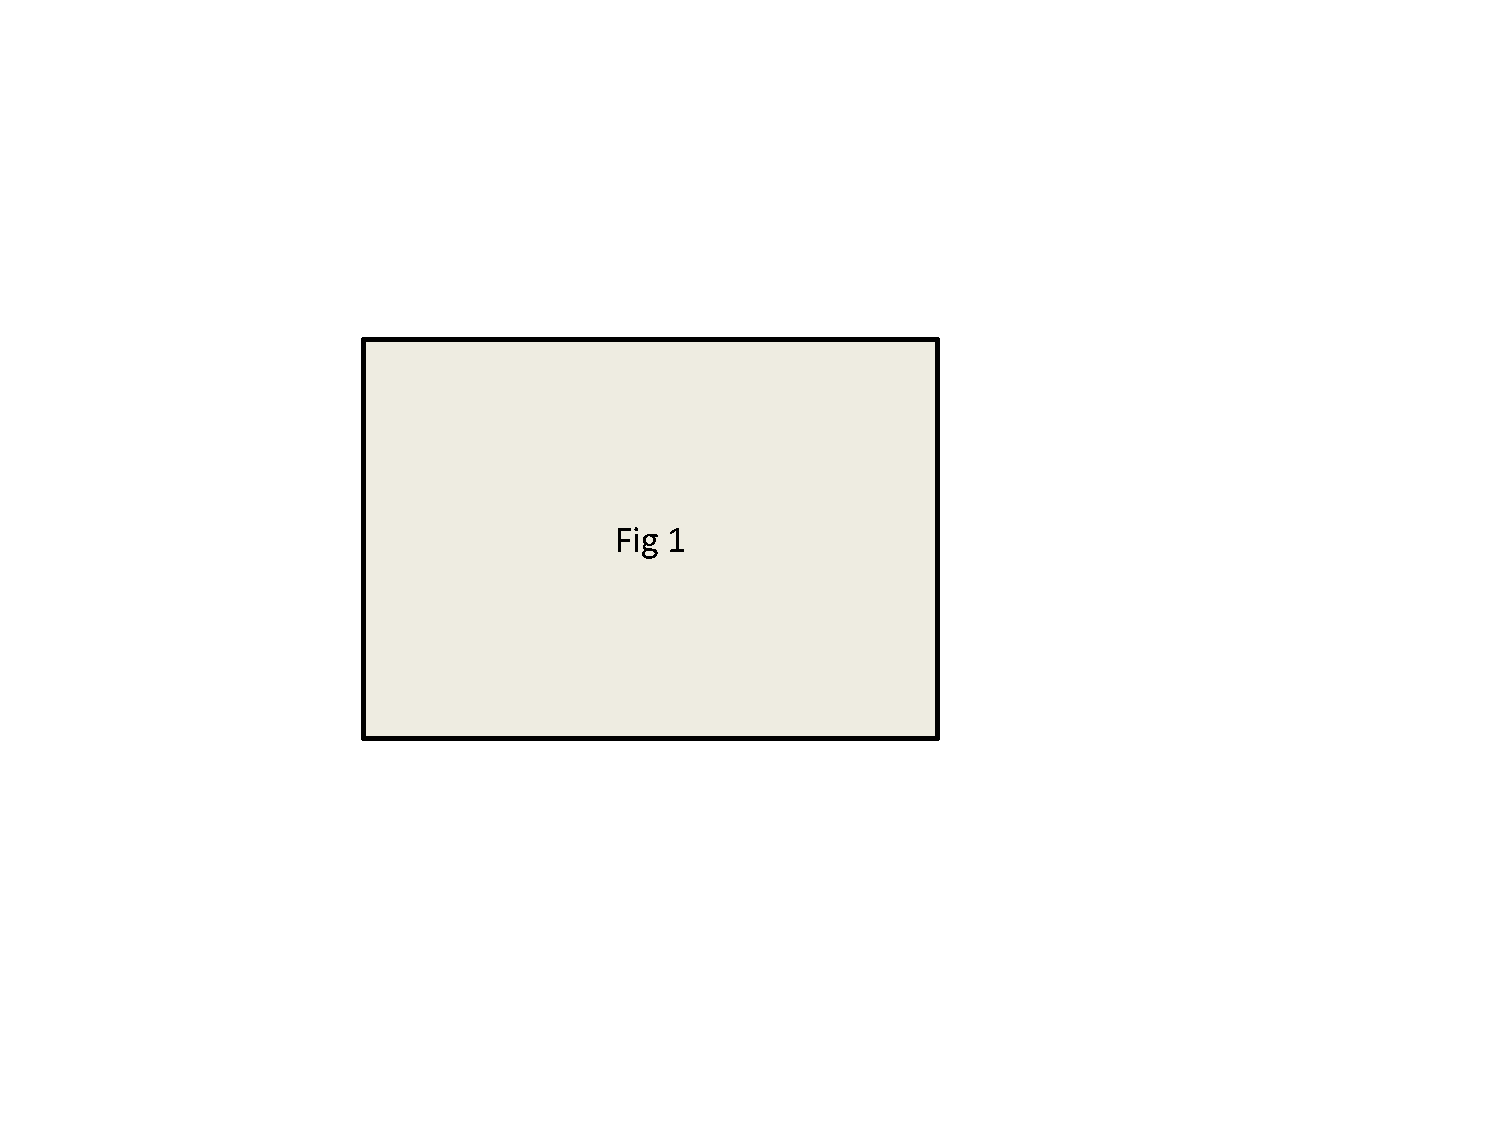
\includegraphics[width=\textwidth]{Fig1.pdf}
  \caption{Sample Figure.}
  \label{fig:Fig1}
\end{figure}


\begin{figure} [!htb]
  \centering
  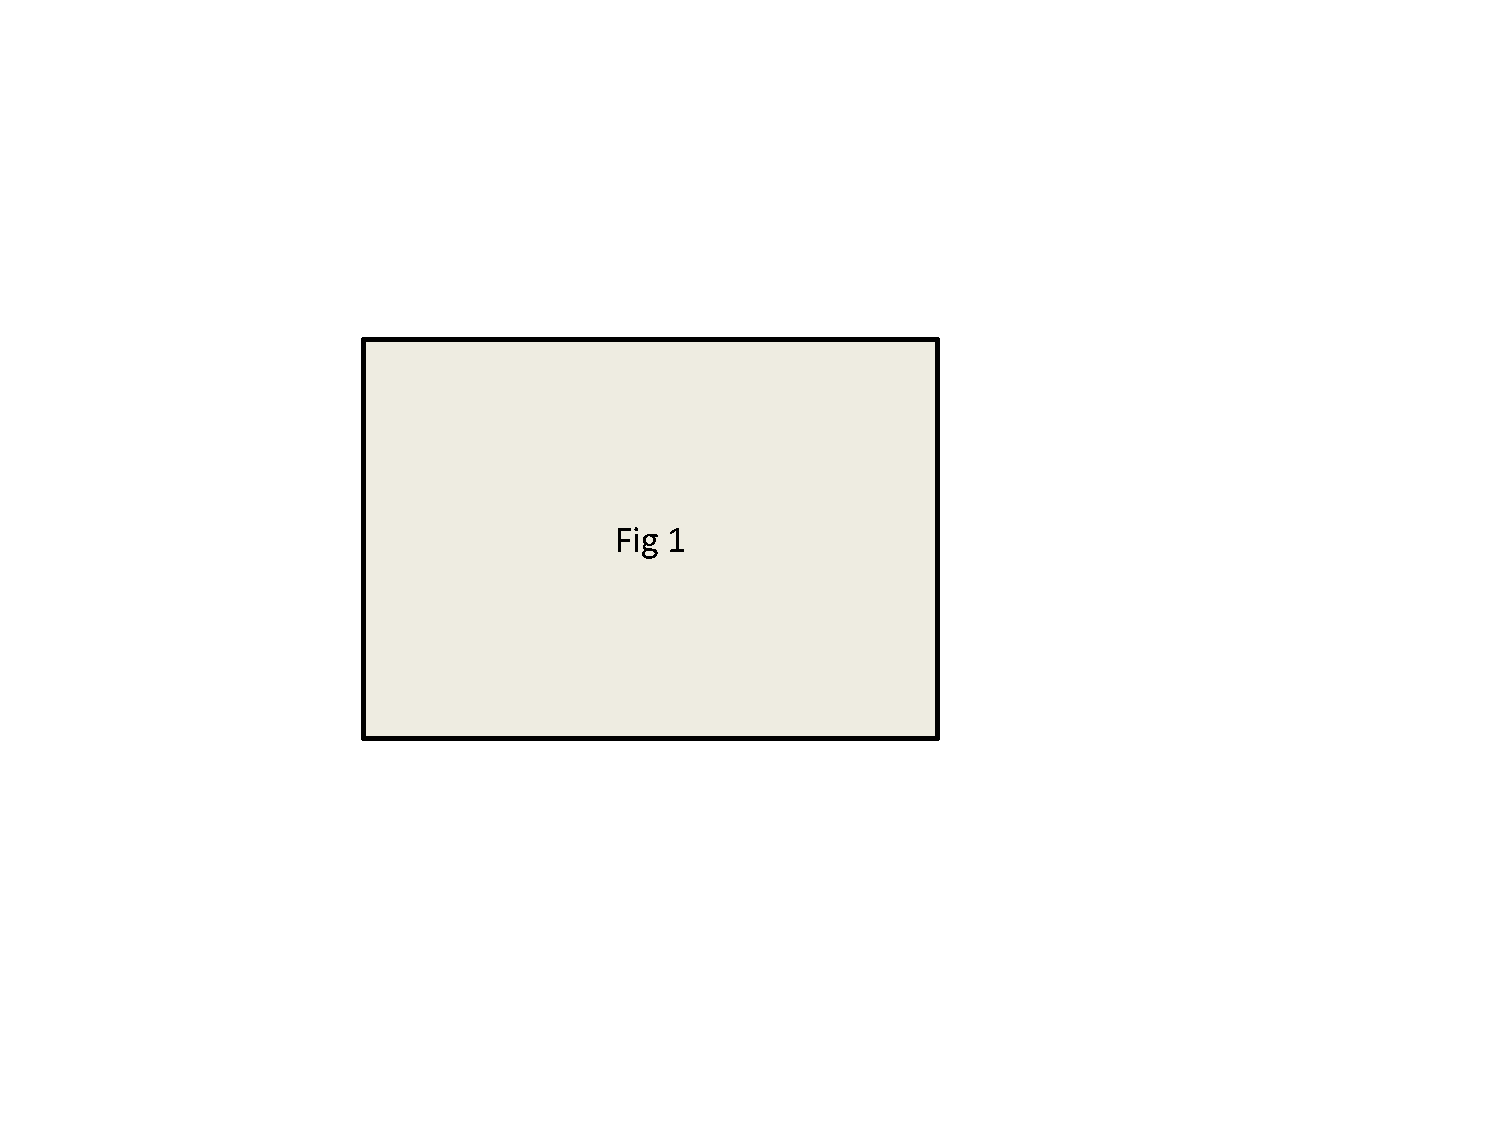
\includegraphics[width=0.3\textwidth]{Fig1.pdf}
 \caption{Sample Smaller Figure.}
  \label{fig:Fig2}
\end{figure}


\subsection{References}

The following sentence demonstrates the usage of references. In Subsection~\ref{sec:figures}) we explained how to use figures in \LaTeX, e.g., Figure~\ref{fig:Fig1}. Don't forget to mention every table, figure or listing you use at least once in your text.

\subsection{Usage of Listings}

\lstset{language=JAVA, breaklines=true, tabsize=2}
\lstinputlisting[caption=HelloWorld,
label=lst:HelloWorld]{listings/HelloWorld.java}



\begin{landscape}

Page in landscape format, e.g., for larger figures or tables; footer remains in portrait format.
\end{landscape}




%%%%%%%%%%%%%%%%%%%%%%%%%%%%%%%%%%%%%%%%%%%%%%%%%%%%%%%%%%%%%%%%%%%%%%%%%%%%%%


%%%%%%%%%%%%%%%%%%%%%%%%%%%%%%%% Conclusion %%%%%%%%%%%%%%%%%%%%%%%%%%%%%%%%%

%%%%%%%%%%%%%%%%%%%%%%%%%%%%%%%%%% Conclusion %%%%%%%%%%%%%%%%%%%%%%%%%%%%%%%%%%%

\chapter{Conclusion}
\label{chap:conclusion}

Lorem ipsum dolor sit amet, consetetur sadipscing elitr, sed diam nonumy eirmod tempor invidunt ut labore et dolore magna aliquyam erat, sed diam voluptua. At vero eos et accusam et justo duo dolores et ea rebum. Stet clita kasd gubergren, no sea takimata sanctus est Lorem ipsum dolor sit amet. Lorem ipsum dolor sit amet, consetetur sadipscing elitr, sed diam nonumy eirmod tempor invidunt ut labore et dolore magna aliquyam erat, sed diam voluptua. At vero eos et accusam et justo duo dolores et ea rebum. Stet clita kasd gubergren, no sea takimata sanctus est Lorem ipsum dolor sit amet.



%%%%%%%%%%%%%%%%%%%%%%%%%%%%%%%%%%%%%%%%%%%%%%%%%%%%%%%%%%%%%%%%%%%%%%%%%%%%%%


%%%%%%%%%%%%%%%%%%%%%%%%%%%%%%%%%%%%%%%%%%%%%%%%%%%%%%%%%%%%%%%%%%%%%%%%%%



%%%%%%%%%%%%%%%%%%%%%%%%% References %%%%%%%%%%%%%%%%%%%%%%%%%%%

\newpage

\phantomsection
\addcontentsline{toc}{chapter}{Appendices}
\appendix
\appendixpage

%%\appendix
%%\phantomsection
%\renewcommand*\appendixpagename{Appendix} 
%%\appendixpage
%%\addappheadtotoc


\chapter{Appendix 1}
\label{chap:appendix_1}

\section{Appendix Section A}
\label{sec:appendix_1}

\section{Appendix Section B}
\label{sec:appendix_2}


\chapter{Appendix 2}
\label{chap:appendix_2}

\clearpage

%%%%%%%%%%%%%%%%%%%%%%%%% Bibliography %%%%%%%%%%%%%%%%%%%%%%%%%%%
\phantomsection
\addcontentsline{toc}{chapter}{Bibliography}
\bibliographystyle{apalike}
\bibliography{References}

\clearpage

%
%%%%%%%%%%%%%%%%%%%%%%%%%%%%%%%%%%%%%%%%%%%%%%%%%%%%%%%%%%%%%%%%%%%%%%%%%%
%% Eidesstattliche Erklärung %%%%
%
% nur bei Abschlussarbeiten! Auch bei englischen Arbeiten auf Deutsch
%

\thispagestyle{empty}
\phantomsection
\label{erklaerung}
%\addcontentsline{toc}{chapter}{Erklärung}
\pdfbookmark[0]{Eidesstattliche Erklärung}{erklaerung}

\setlength{\parindent}{0em}

\markboth{\uppercase{Eidesstattliche Erklärung}}{}
\textbf{\large{Erklärung an Eides statt}}

 \vspace*{65pt}
 
%% WICHTIG: unpassendes rauslöschen, sodass nur EINE Erklärung in der Arbeit steht 

%% Bachelor und Master nach Prüfungsordnung 2015
%\vspace*{20pt}
Ich habe die vorliegende Arbeit selbstständig verfasst und keine anderen als die angegebenen Quellen und Hilfsmittel benutzt. Die Arbeit wurde bisher an keiner anderen Hochschule zur Erlangung eines akademischen Grades eingereicht. Die vorgelegten Druckexemplare und die dem Prüfer / der Prüferin zur Verfügung gestellte elektronische Version (PDF-Datei) der Arbeit sind identisch. Von den in §13 Abs. 3 PO 2015 vorgesehenen Rechtsfolgen habe ich Kenntnis.

%% Bachelor nach Prüfungsordnung 2021
Ich habe die vorliegende Arbeit selbstständig verfasst und keine anderen als die angegebenen Quellen und Hilfsmittel benutzt. Die Arbeit wurde bisher an keiner anderen Hochschule zur Erlangung eines akademischen Grades eingereicht. Die vorgelegten Druckexemplare und die dem Prüfer / der Prüferin zur Verfügung gestellte elektronische Version (PDF-Datei) der Arbeit sind identisch. Von den in §27 Abs. 6 BPO 2021 vorgesehenen Rechtsfolgen habe ich Kenntnis.

\vspace*{65pt}

%% Master nach Prüfungsordnung 2021
Ich habe die vorliegende Arbeit selbstständig verfasst und keine anderen als die angegebenen Quellen und Hilfsmittel benutzt. Die Arbeit wurde bisher an keiner anderen Hochschule zur Erlangung eines akademischen Grades eingereicht. Die vorgelegten Druckexemplare und die dem Prüfer / der Prüferin zur Verfügung gestellte elektronische Version (PDF-Datei) der Arbeit sind identisch. Von den in §26 Abs. 6 MPO 2021 vorgesehenen Rechtsfolgen habe ich Kenntnis.

\vspace*{65pt}

Regensburg, den \submissiondate

\vspace*{60pt}


\authorname

Matrikelnummer \studentID

\end{document}
